\documentclass{beamer}
\usepackage{beamerthemeshadow}
\usepackage{color}
\usepackage[all]{xy}



\mode<presentation>
{
  \usetheme{Warsaw} %%% Change later
 \usecolortheme{dove}


  \setbeamercovered{transparent}
  % or whatever (possibly just delete it)
}
\setbeamertemplate{footline}[page number]{}


\begin{document}
\title{Use of Clojure in Undergraduate CS Curriculum}
\author{Elena Machkasova}
\institute[UMM] % (optional, but mostly needed)
{
 % \inst{1}%
  University of Minnesota, Morris
}
\date[]  
{ Boston Clojure meetup, November 8, 2012.}

\begin{frame}
  \titlepage
\end{frame}

\begin{frame}

  \frametitle{Outline}
\tableofcontents
\end{frame}

\section{UMM CS program}

\begin{frame}
  \frametitle{What is University of Minnesota, Morris?}
{\center \qquad \qquad \quad
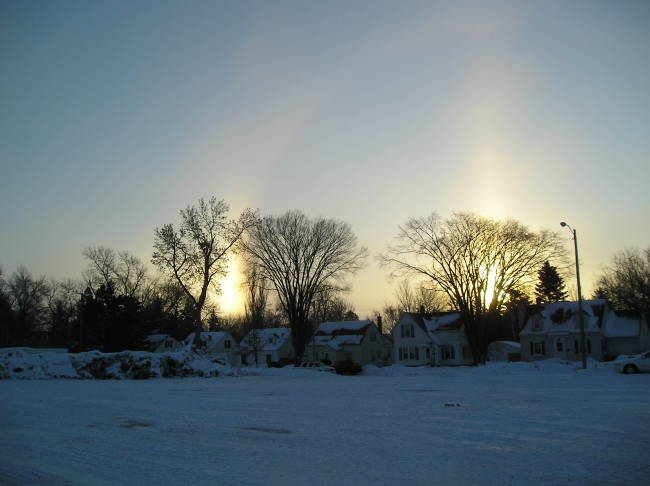
\includegraphics[height=45mm]{halo.jpg}
}

UMM: small public undergraduate liberal arts college in rural MN.
\begin{itemize}
\item a campus of UMN, 3.5 hrs away from Twin Cities. 
\item town of 5000 people, amidst corn fields and cows. 
\item $<$ 2000 students (15-20 CS majors per year)
\end{itemize}
%%%{\tt there will be a picture}

\end{frame}

\subsection{About UMM CS}

\begin{frame}
  \frametitle{Why UMM?}
\begin{itemize}
%%% Want to make these appear one by one %%%%%%%%%%%%%%%%
\item Functional language in intro class (Scheme).
\item Combination of in-depth theory with new technologies (emphasis on testing, group work support).
\item Openness to new technologies and ideas.
\item Close connections and collaboration between faculty, students, and alums. 
\item Small group of dedicated faculty. 
%\item Research with undergraduates
%\item Lots of responsibility to undergraduates (lab admin, committees)
%\item A small number of dedicated faculty
%\item Close connections to alums
\end{itemize}
\end{frame}

\begin{frame}
  \frametitle{Structure of CS program (partial)}
{\small
\xymatrix{
*\txt{Intro to CS\\ (Scheme/Python)}\ar@{-->}[dr] &  & *\txt{Discrete Math}\ar@{-->}[ddl] \\
&*\txt{Data Structures \\ (Java)}\ar@{-->}[dl]\ar@{-->}[d]\ar@{-->}[dr] \\
*\txt{Software Design}\ar@{-->}[d] & *\txt{Algorithms}\ar@{-->}[d] & *\txt{Intro~to~Systems}\ar@{-->}[d] \\
*\txt{Elective (P\&L)} & *\txt{Elective (Theory)} & *\txt{Elective (Systems)}
}
}
\end{frame}

\subsection{Clojure at UMM}

\begin{frame}
  \frametitle{Clojure in CS at UMM}
%%%% Break into two slides
Timeline: 
\begin{itemize}
\item 2010: Brian Goslinga (UMM CS'11) mentioned Clojure to faculty.
\item Spring 2011: {\it Programming for Parallel Architecture} class explored Clojure, Erlang, and Hadoop. 
\item Spring 2011:  A one-semester project on improving Clojure error messages. 
\item Spring 2012: Used Clojure in {\it Programming Languages} class: as an example of a Lisp and as a language for concurrency.  
\item Stephen Adams (UMM CS'12): a one-semester project on integrating Clojure and Java, with the idea of integrating Clojure into Data Structure. %%%%%%%%%%%%%%{\tt perhaps not to include?}  
\item Spring 2012: Decision to change our intro class to Clojure. %%%%%%%%%% Thanks to ... for suggestions on libraries, etc.
\end{itemize}
\end{frame}

\begin{frame}
  \frametitle{Where the new Clojure class belongs}
{\small
\xymatrix{
*\txt{\alert{Intro to CS}\\ (\alert{Clojure}/Python)}\ar@{-->}[dr] &  & *\txt{Discrete Math}\ar@{-->}[ddl] \\
&*\txt{Data Structures \\ (Java)}\ar@{-->}[dl]\ar@{-->}[d]\ar@{-->}[dr] \\
*\txt{Software Design}\ar@{-->}[d] & *\txt{Algorithms}\ar@{-->}[d] & *\txt{Intro~to~Systems}\ar@{-->}[d] \\
*\txt{Elective (P\&L)} & *\txt{Elective (Theory)} & *\txt{Elective (Systems)}
}
}
\end{frame}

\begin{frame}
  \frametitle{Clojure in CS at UMM}
%%%% Break into two slides
Timeline (cont.):
\begin{itemize} 
\item Fall 2012: a directed study (Joe Einertson, UMM CS'13) on developing a Clojure programming environment for novice students.
\item Spring 2013: a directed study on creating sample exercises and improving the environment. 
\item Fall 2013: the first offering of the new class. 
\item ...Possibly incorporating Clojure into Data Structures and/or Software Design? Web development? Concurrency? 
\item ...Possibly a textbook? 
\end{itemize}
\end{frame}

\section{Introductory class in Clojure}

\subsection{Current intro class}

\begin{frame}
  \frametitle{The introductory class}
Problem Solving and Algorithm Development. \\[1.2ex]

4 credits (roughly 3 in-class hours, no allocated lab time) \\[2ex]

{\it Course description: }Introduction to problem solving approaches, major programming paradigms, hardware, software, and data representations. Study of the functional programming paradigm, concentrating on recursion and inductively-defined data structures. Simple searching and sorting algorithms.
Prerequisites: none. 
\end{frame}

\begin{frame}
  \frametitle{Why a functional language in an intro CS class?}
Why teach a functional language in an intro class if mostly imperative languages are used later? 
\begin{itemize}
\item Better understanding of recursion (useful for recursive data structures, e.g. binary trees, and recursive algorithms, e.g. sorting)
\item Focus on functions.
\item Focus on abstraction, generalization, and modularity. 
\end{itemize}
\end{frame}


\begin{frame}
  \frametitle{Current intro class at UMM}
Currently use How to Design Programs (HtDP) curriculum developed by Matthias Felleisen, Robert Bruce Findler, Matthew Flatt, Shriram Krishnamurthi. 
\begin{itemize}
\item 35+ students. 
\item Language: Racket (a version of Scheme).
\item Environment: DrRacket. Features several language levels (Beginner $\to$ Advanced), libraries for incorporating graphics and interaction. 
\item Online textbook, series of exercises.
\item A large scale open-ended group exercise: develop a game. Interactive, somewhat competitive. Allows students to explore the language and practice/develop design techniques. 
\end{itemize}
%%%{\tt add a picture}
\end{frame}

\subsection{Goals and challenges of teaching Clojure in intro class}

\begin{frame}
  \frametitle{Why Clojure in an intro CS class?}
Benefits from switching to Clojure:
\begin{itemize}
\item Used in industry.
\item Interoperability with Java. 
\item Concurrency features. 
\item Efficiency.
\item {\it More?}
\end{itemize}
\end{frame}


\begin{frame}
  \frametitle{Challenges in introducing Clojure}
Challenges:
\begin{itemize}
\item HtDP framework is hard to beat.
\item HtDP framework is hard not to repeat - how do we teach Clojure and not Racket?
\item Purely functional vs state? 
\item How much concurrency do we include? 
\item Environment for new students (convenience, tracing a program, graphics).
\item Error messages!!!
\item Using off-the-shelf libraries and tools.
\end{itemize}
\end{frame}

\section{Clojure setup}

\subsection{Tools and programming environment}

\begin{frame}
  \frametitle{Libraries and tools}
What we are planning to use :
\begin{itemize}
\item Turtle graphics.
\item Seesaw (Clojure abstraction over Java Swing) .
\item Testing (still to be decided), use of pre- and post-conditions. 
\end{itemize}
What we aren't planning to use in the intro class:
\begin{itemize}
\item web dev, including ClojureScript. Introducing web dev concepts would take too much time and distract from the educational goals of the class. 
\end{itemize}
Thanks to Jon Anthony, Brian Goslinga, and Stephen Adams for helpful suggestions and discussions!
\end{frame}

\begin{frame}
  \frametitle{Programming environment}
Goals:
\begin{itemize}
\item Cross-platform (Linux in the lab, Windows, Mac).
\item Easy for novice programmers.
\item Access to REPL, easy/fast reloading of student code. 
\item Some way to trace the program. 
\item The ability to pre-package some libraries and abstract over project management. 
\item Reasonably easy maintenance (version updates, library updates, etc). 
\end{itemize}
\end{frame}

\begin{frame}
  \frametitle{Programming environment (cont.)}
Possible setups:
\begin{itemize}
\item jEdit  (with ClojureShell and LispIndent plugins) +  leiningen. {\it How do we reload code fast?}
\item Light Table IDE - a kickstarter project, under development
\end{itemize}
We are not considering:
\begin{itemize}
\item Eclipse with Counterclockwise (too many unclear options, too slow), 
\item emacs or vim (too confusing to new students). 
\end{itemize}
%%%%{\tt perhaps screen shots or examples for jEdit}
\end{frame}

\begin{frame}
  \frametitle{Tracing a program}
Options for step-by-step execution:
\begin{itemize}
\item dotrace and such,
\item {\tt slingshot} - enhances exceptions (can throw any object; could be used for reporting program execution),
\item {\tt spyscope} - a library designed for debugging single- and multi-threaded applications. 
\item Light Table does some tracing automagically. 
\end{itemize}
Still need to look more into it, depends on the choice of IDE. 
\end{frame}

\subsection{Improving error messages}

\begin{frame}[fragile]
  \frametitle{Error messages: unreadable and unhelpful for new programmers}
Passing a number instead of a function: {\tt (map 2 [1 2 3])}
{\tiny
\begin{verbatim}
(Exception in thread "main" java.lang.ClassCastException: java.lang.Long cannot
be cast to clojure.lang.IFn
        at clojure.core$map$fn__4182.invoke(core.clj:2469)
        at clojure.lang.LazySeq.sval(LazySeq.java:42)
        at clojure.lang.LazySeq.seq(LazySeq.java:60)
        at clojure.lang.RT.seq(RT.java:474)
        at clojure.core$seq.invoke(core.clj:133)
        at clojure.core$print_sequential.invoke(core_print.clj:46)
        at clojure.core$fn__5378.invoke(core_print.clj:143)
        at clojure.lang.MultiFn.invoke(MultiFn.java:231)
        at clojure.core$pr_on.invoke(core.clj:3306)
        at clojure.core$pr.invoke(core.clj:3318)
        at clojure.lang.AFn.applyToHelper(AFn.java:161)
        at clojure.lang.RestFn.applyTo(RestFn.java:132)
        at clojure.core$apply.invoke(core.clj:614)
        at clojure.core$prn.doInvoke(core.clj:3351)
        at clojure.lang.RestFn.invoke(RestFn.java:408)
        at clojure.main$eval_opt.invoke(main.clj:299)
       ...
        at clojure.lang.RestFn.invoke(RestFn.java:421)
        at clojure.lang.Var.invoke(Var.java:419)
        at clojure.lang.AFn.applyToHelper(AFn.java:163)
        at clojure.lang.Var.applyTo(Var.java:532)
        at clojure.main.main(main.java:37)
\end{verbatim}
}
\end{frame}

\begin{frame}
  \frametitle{Improving error messages}
Our approach to improving error messages:
\begin{itemize}
\item Filtering the stack. 
\item Wrapping common functions (e.g. map) into pre-conditions with meaningful naming. 
\item Dictionary of common messages.
\end{itemize}
Work in progress, by Joe Einertson (UMM CS'13) and myself. The pre-conditions idea is due to Joe. 
\end{frame}


\begin{frame}
  \frametitle{Filtering the stack}
\begin{itemize}
\item {\tt clj-stacktrace} library gives access to stack trace info. 
\item Filter out everything that starts with {\tt clojure} and {\tt java}. More fine-grained and customizable filtering would be preferred eventually. {\it Any pointers on converting between namespaces and package names?}
\item surround all student code with {\tt try/catch}, catch exceptions, pass through a filtering/prettifying function. 
\end{itemize}
%%%{\tt Options, ideally customizable, example}
\end{frame}

\begin{frame}[fragile]
  \frametitle{Pre-conditions for error messages}
%\begin{itemize}
Wrap functions in {\tt clojure.core} in our function with a pre-condition:
\begin{verbatim}
(ns corefns.core
(:refer-clojure :exclude [map])) ; can't overwrite core 

(def is-function? fn?)
(def is-collection? coll?)

(defn map [argument1 argument2]
{:pre[(is-function? argument1)(is-collection? argument2)]}
  (clojure.core/map argument1 argument2))
\end{verbatim}
%\end{itemize}
%{\tt pre-conditions, try/catch, all the plugins}
\end{frame}

\begin{frame}[fragile]
  \frametitle{Sample error messages}
%\begin{itemize}
Wrong number of arguments: {\tt (map [1 2 3])}
\begin{verbatim}
ERROR: Wrong number of args (1) passed to: core$map
Possible causes:
        intro.core/-main (core.clj line 45)
        user/eval5273 (NO_SOURCE_FILE line 1)
\end{verbatim}
Wrong type: {\tt (map 2 [1 2 3])}
\begin{verbatim}
ERROR: Assert failed: (is-function? argument1)
Possible causes:
        corefns.core/map (core.clj line 9)
        intro.core/-main (core.clj line 44)
        user/eval5273 (NO_SOURCE_FILE line 1)
\end{verbatim}
%\end{itemize}
%{\tt pre-conditions, try/catch, all the plugins}
\end{frame}

\begin{frame}[fragile]
  \frametitle{Dictionary of common messages}
%%%{\tt Options, ideally customizable, example}
Messages are still confusing: {\tt (2 + 3)}
\begin{verbatim} 
ERROR: java.lang.Long cannot be cast to clojure.lang.IFn
Possible causes:
        intro.core/-main (core.clj line 44)
        user/eval5273 (NO_SOURCE_FILE line 1)
\end{verbatim}
Possible meaning: you are using a number in place of a function or an operation. 

Ideally would like to remind about the prefix notation. Work for the Directed Study class in the Spring. 
\end{frame}


%%%\section{Clojure is not Racket}

\begin{frame}
  \frametitle{Clojure is not Racket}
What Clojure-specific features do we teach? 
\begin{itemize}
\item Pre- and post-conditions; how do they coexist with testing? What testing framework?
\item How much of state do we show and explain? atoms, refs, STM, etc? To which degree do we abstract over state? 
\item Concurrency: how much of automagical parallelism (pmap and friends) can we show/use? 
\item How much of Java interops do we show/use?
\end{itemize}
Conflicting goals: focus on nice clean functional code vs learning the real useful language. Can we do both? 
\end{frame}


\section{Future steps}

\begin{frame}
  \frametitle{Introductory class}
Future work for the introductory class:
\begin{itemize}
\item Finalize the environment, fill in the gaps (error message dictionary, etc.).
\item Examples, exercises, notes. 
\item How much state, how much concurrency?
\item Fall 2013: teach the class.
\item Assessment, modify notes, perhaps a textbook?
\end{itemize}
\end{frame}

\begin{frame}
  \frametitle{Other classes}
Possible other classes to incorporate Clojure:
\begin{itemize}
\item {\it Data Structures:} currently Java, mutable structures (for the most part). Possibly: functional structures, mix of Java and Clojure. 
\item  {\it Software Design and Development:} abstracting over Swing with Seesaw, web dev stuff (ClojureScript, web framework). 
\item {\it Web programming courses:} see above. 
\item {\it Parallel/distributed algorithms and systems:} {\tt pmap} and friends. 
\end{itemize}
Challenge: not all students would go through Clojure intro class. 
\end{frame}

\begin{frame}
  \frametitle{Other classes that could include Clojure}
{\small
\xymatrix{
*\txt{\alert{Intro to CS}\\ (\alert{Clojure}/Python)}\ar@{-->}[dr] &  & *\txt{Discrete Math}\ar@{-->}[ddl] \\
&*\txt{\alert{Data Structures} \\ (Java/\alert{Clojure})}\ar@{-->}[dl]\ar@{-->}[d]\ar@{-->}[dr] \\
*\txt{\alert{Software Design}}\ar@{-->}[d] & *\txt{Algorithms}\ar@{-->}[d] & *\txt{Intro~to~Systems}\ar@{-->}[d] \\
*\txt{\alert{Elective (P\&L)}\\\alert{Web dev}} & *\txt{Elective (Theory)} & *\txt{\alert{Elective (Systems)}\\\alert{concurrency}}
}
}
\end{frame}

\begin{frame}
  \frametitle{Any suggestions?}
\begin{itemize}
\item What is a fast way of reloading a file in REPL? Restarting the JVM takes forever. Currently we: remove the namespace, reload the file, then do {\tt in-ns}.
\item Are there tools for converting between namespaces and package/class names? 
\end{itemize}
\end{frame}

\begin{frame}
  \frametitle{Discussion}
Questions? Suggestions? Comments? Critique? 
\end{frame}

\end{document}

